%
% $RCSfile: pipes_and_filters.tex,v $
%
% Copyright (c) 2004. Christian Heller. All rights reserved.
%
% No copying, altering, distribution or any other actions concerning this
% document, except after explicit permission by the author!
% At some later point in time, this document is planned to be put under
% the GNU FDL license. For now, _everything_ is _restricted_ by the author.
%
% http://www.cybop.net
% - Cybernetics Oriented Programming -
%
% http://www.resmedicinae.org
% - Information in Medicine -
%
% @author Christian Heller <christian.heller@tuxtax.de>
%

\paragraph{Pipes and Filters}
\label{pipes_and_filters_heading}

Systems that process streams of data may use the \emph{Pipes and Filters}
pattern \cite{buschmann}. It encapsulates every processing step in an own
\emph{Filter} component and forwards the data through channels which are called
\emph{Pipeline} (figure \ref{pipesfilters_figure}). Families of related systems
can be formed by changing the single filter positions. The data forwarding can
follow various scenarios:

\begin{itemize}
    \item[-] \emph{Push:} active filter pushes data to passive filter
    \item[-] \emph{Pull:} active filter pulls data from passive filter
    \item[-] \emph{Mixed Push-Pull-Pipeline:} all filters push or pull data
    \item[-] \emph{Independent Loops:} all filters actively access pipeline
\end{itemize}

\begin{figure}[ht]
    \begin{center}
        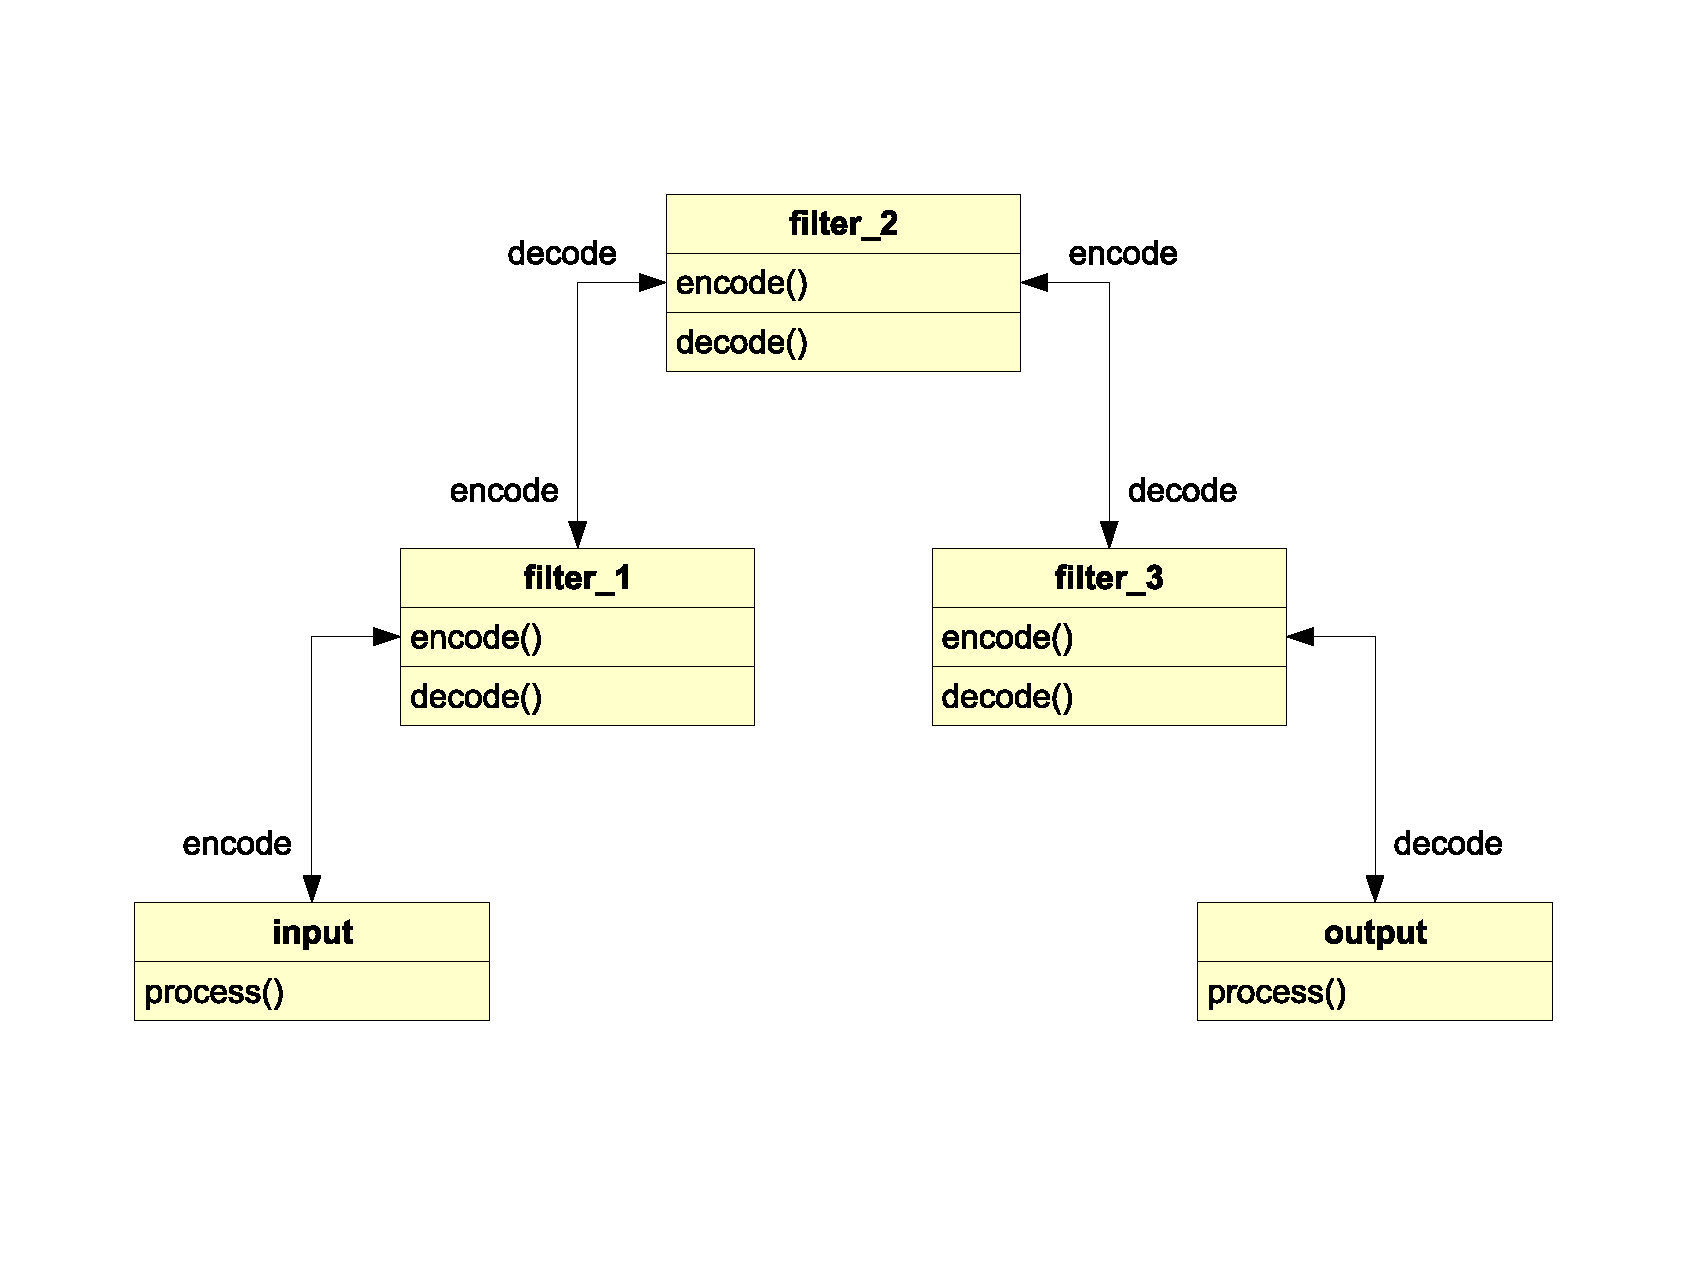
\includegraphics[scale=0.3]{vector/pipesfilters.eps}
        \caption{Pipes and Filters Pattern}
        \label{pipesfilters_figure}
    \end{center}
\end{figure}
